\documentclass[
  shownotes,
  xcolor={svgnames},
  hyperref={colorlinks,citecolor=DarkBlue,linkcolor=DarkRed,urlcolor=DarkBlue}
  , aspectratio=169]{beamer}
\usepackage{animate}
\usepackage{amsmath}
\usepackage{amsfonts}
\usepackage{amssymb}
\usepackage{pifont}
\usepackage{mathpazo}
%\usepackage{xcolor}
\usepackage{multimedia}
\usepackage{fancybox}
\usepackage[para]{threeparttable}
\usepackage{multirow}
\setcounter{MaxMatrixCols}{30}
\usepackage{subcaption}
\usepackage{graphicx}
\usepackage{lscape}
\usepackage[compatibility=false,font=small]{caption}
\usepackage{booktabs}
\usepackage{ragged2e}
\usepackage{chronosys}
\usepackage{appendixnumberbeamer}
\usepackage{animate}
\setbeamertemplate{caption}[numbered]
\usepackage{color}
%\usepackage{times}
\usepackage{tikz}
\usepackage{comment} %to comment
%% BibTeX settings
\usepackage{natbib}
\bibliographystyle{apalike}
\bibpunct{(}{)}{,}{a}{,}{,}
\setbeamertemplate{bibliography item}{[\theenumiv]}

% Defines columns for bespoke tables
\usepackage{array}
\newcolumntype{L}[1]{>{\raggedright\let\newline\\\arraybackslash\hspace{0pt}}m{#1}}
\newcolumntype{C}[1]{>{\centering\let\newline\\\arraybackslash\hspace{0pt}}m{#1}}
\newcolumntype{R}[1]{>{\raggedleft\let\newline\\\arraybackslash\hspace{0pt}}m{#1}}


\usepackage{xfrac}


\usepackage{multicol}
\setlength{\columnsep}{0.5cm}

% Theme and colors
\usetheme{Boadilla}

% I use steel blue and a custom color palette. This defines it.
\definecolor{andesred}{HTML}{af2433}

% Other options
\providecommand{\U}[1]{\protect\rule{.1in}{.1in}}
\usefonttheme{serif}
\setbeamertemplate{itemize items}[default]
\setbeamertemplate{enumerate items}[square]
\setbeamertemplate{section in toc}[circle]

\makeatletter

\definecolor{mybackground}{HTML}{82CAFA}
\definecolor{myforeground}{HTML}{0000A0}

\setbeamercolor{normal text}{fg=black,bg=white}
\setbeamercolor{alerted text}{fg=red}
\setbeamercolor{example text}{fg=black}

\setbeamercolor{background canvas}{fg=myforeground, bg=white}
\setbeamercolor{background}{fg=myforeground, bg=mybackground}

\setbeamercolor{palette primary}{fg=black, bg=gray!30!white}
\setbeamercolor{palette secondary}{fg=black, bg=gray!20!white}
\setbeamercolor{palette tertiary}{fg=white, bg=andesred}

\setbeamercolor{frametitle}{fg=andesred}
\setbeamercolor{title}{fg=andesred}
\setbeamercolor{block title}{fg=andesred}
\setbeamercolor{itemize item}{fg=andesred}
\setbeamercolor{itemize subitem}{fg=andesred}
\setbeamercolor{itemize subsubitem}{fg=andesred}
\setbeamercolor{enumerate item}{fg=andesred}
\setbeamercolor{item projected}{bg=gray!30!white,fg=andesred}
\setbeamercolor{enumerate subitem}{fg=andesred}
\setbeamercolor{section number projected}{bg=gray!30!white,fg=andesred}
\setbeamercolor{section in toc}{fg=andesred}
\setbeamercolor{caption name}{fg=andesred}
\setbeamercolor{button}{bg=gray!30!white,fg=andesred}


\usepackage{fancyvrb}
\newcommand{\VerbBar}{|}
\newcommand{\VERB}{\Verb[commandchars=\\\{\}]}
\DefineVerbatimEnvironment{Highlighting}{Verbatim}{commandchars=\\\{\}}
% Add ',fontsize=\small' for more characters per line
\usepackage{framed}
\definecolor{shadecolor}{RGB}{248,248,248}
\newenvironment{Shaded}{\begin{snugshade}}{\end{snugshade}}
\newcommand{\AlertTok}[1]{\textcolor[rgb]{0.94,0.16,0.16}{#1}}
\newcommand{\AnnotationTok}[1]{\textcolor[rgb]{0.56,0.35,0.01}{\textbf{\textit{#1}}}}
\newcommand{\AttributeTok}[1]{\textcolor[rgb]{0.77,0.63,0.00}{#1}}
\newcommand{\BaseNTok}[1]{\textcolor[rgb]{0.00,0.00,0.81}{#1}}
\newcommand{\BuiltInTok}[1]{#1}
\newcommand{\CharTok}[1]{\textcolor[rgb]{0.31,0.60,0.02}{#1}}
\newcommand{\CommentTok}[1]{\textcolor[rgb]{0.56,0.35,0.01}{\textit{#1}}}
\newcommand{\CommentVarTok}[1]{\textcolor[rgb]{0.56,0.35,0.01}{\textbf{\textit{#1}}}}
\newcommand{\ConstantTok}[1]{\textcolor[rgb]{0.00,0.00,0.00}{#1}}
\newcommand{\ControlFlowTok}[1]{\textcolor[rgb]{0.13,0.29,0.53}{\textbf{#1}}}
\newcommand{\DataTypeTok}[1]{\textcolor[rgb]{0.13,0.29,0.53}{#1}}
\newcommand{\DecValTok}[1]{\textcolor[rgb]{0.00,0.00,0.81}{#1}}
\newcommand{\DocumentationTok}[1]{\textcolor[rgb]{0.56,0.35,0.01}{\textbf{\textit{#1}}}}
\newcommand{\ErrorTok}[1]{\textcolor[rgb]{0.64,0.00,0.00}{\textbf{#1}}}
\newcommand{\ExtensionTok}[1]{#1}
\newcommand{\FloatTok}[1]{\textcolor[rgb]{0.00,0.00,0.81}{#1}}
\newcommand{\FunctionTok}[1]{\textcolor[rgb]{0.00,0.00,0.00}{#1}}
\newcommand{\ImportTok}[1]{#1}
\newcommand{\InformationTok}[1]{\textcolor[rgb]{0.56,0.35,0.01}{\textbf{\textit{#1}}}}
\newcommand{\KeywordTok}[1]{\textcolor[rgb]{0.13,0.29,0.53}{\textbf{#1}}}
\newcommand{\NormalTok}[1]{#1}
\newcommand{\OperatorTok}[1]{\textcolor[rgb]{0.81,0.36,0.00}{\textbf{#1}}}
\newcommand{\OtherTok}[1]{\textcolor[rgb]{0.56,0.35,0.01}{#1}}
\newcommand{\PreprocessorTok}[1]{\textcolor[rgb]{0.56,0.35,0.01}{\textit{#1}}}
\newcommand{\RegionMarkerTok}[1]{#1}
\newcommand{\SpecialCharTok}[1]{\textcolor[rgb]{0.00,0.00,0.00}{#1}}
\newcommand{\SpecialStringTok}[1]{\textcolor[rgb]{0.31,0.60,0.02}{#1}}
\newcommand{\StringTok}[1]{\textcolor[rgb]{0.31,0.60,0.02}{#1}}
\newcommand{\VariableTok}[1]{\textcolor[rgb]{0.00,0.00,0.00}{#1}}
\newcommand{\VerbatimStringTok}[1]{\textcolor[rgb]{0.31,0.60,0.02}{#1}}
\newcommand{\WarningTok}[1]{\textcolor[rgb]{0.56,0.35,0.01}{\textbf{\textit{#1}}}}
\usepackage{graphicx}
\makeatletter


% colors
\definecolor{airforceblue}{rgb}{0.36, 0.54, 0.66}
\newcommand{\theme}{\color{andesred}}
\newcommand{\bk}{\color{black}}
\newcommand{\rd}{\color{red}}
\newcommand{\fg}{\color{ForestGreen}}
\newcommand{\bl}{\color{blue}}
\newcommand{\gr}{\color{black!60}}
\newcommand{\sg}{\color{DarkSlateGray}}
\newcommand{\br}{\color{SaddleBrown}}
\newcommand{\nv}{\color{Navy}}


% common math markups
\newcommand{\bs}[1]{\boldsymbol{#1}}
\newcommand{\mc}[1]{\mathcal{#1}}
\newcommand{\mr}[1]{\mathrm{#1}}
\newcommand{\bm}[1]{\mathbf{#1}}
\newcommand{\ds}[1]{\mathds{#1}}
\newcommand{\indep}{\perp\!\!\!\perp}

% shorthand
\newcommand{\sk}{\vspace{.5cm}}
\newcommand{\R}[1]{{\tt \nv #1}}
\newcommand{\til}{{\footnotesize$\bs{\stackrel{\sim}{}}$}}
\DeclareSymbolFont{extraup}{U}{zavm}{m}{n}
\DeclareMathSymbol{\vardiamond}{\mathalpha}{extraup}{87}


\usepackage{tikz}
% Tikz settings optimized for causal graphs.
\usetikzlibrary{shapes,decorations,arrows,calc,arrows.meta,fit,positioning}
\tikzset{
    -Latex,auto,node distance =1 cm and 1 cm,semithick,
    state/.style ={ellipse, draw, minimum width = 0.7 cm},
    point/.style = {circle, draw, inner sep=0.04cm,fill,node contents={}},
    bidirected/.style={Latex-Latex,dashed},
    el/.style = {inner sep=2pt, align=left, sloped}
}


\makeatother






%%%%%%%%%%%%%%% BEGINS DOCUMENT %%%%%%%%%%%%%%%%%%

\begin{document}
 
\title[Lecture 27]{Lecture 27:  Text as Data}
\subtitle{Big Data and Machine Learning for Applied Economics \\ Econ 4676}
\date{\today}

\author[Sarmiento-Barbieri]{Ignacio Sarmiento-Barbieri}
\institute[Uniandes]{Universidad de los Andes}


\begin{frame}[noframenumbering]
\maketitle
\end{frame}

%%%%%%%%%%%%%%%%%%%%%%%%%%%%%%%%%%%


%----------------------------------------------------------------------% 

\begin{frame}
\frametitle{Announcements}

\begin{itemize}
\item Problem Set 3: Check the data set, I changed it. I had forgotten a variable {\tt Npobres}. You can still use the previous one to train the model. But the submission should be with the new data set.
\medskip
\item The submission of the .csv is on Wednesday at November 18 at 8:00 pm. Please send it via slack with the number of paramters in your model. If you forget to send me the number of parameters I'll assign $100,000$
\medskip
\item We need to decide the Final Exam Window: I posted a poll. Possible dates
\begin{itemize}
  \item December 3 from 2pm (Thursday) to December 5 2pm (Saturday) (preferred)
  \item December 7 from 8am (Monday) to December 9 8am (Wednesday)
  \item December 9 from 8am (Wednesday) to December 11 8am (Friday)
  \item If none of these work we can tweak them a little bit

\end{itemize}
\end{itemize}

\end{frame}

%----------------------------------------------------------------------% 

\begin{frame}
\frametitle{Agenda}

\tableofcontents

\end{frame}
%----------------------------------------------------------------------%
\section{Recap: XGBoost}
%----------------------------------------------------------------------%

%----------------------------------------------------------------------%
\begin{frame}[fragile]
\frametitle{XGBoost: Demo}
\begin{itemize}
\item From \texttt{Caret's} manual

\item eXtreme Gradient Boosting
\medskip
\begin{itemize}
\item method = `xgbTree'
\medskip
\item Type: Regression, Classification
\medskip
\item Tuning parameters:

  
  \begin{verbatim}
  nrounds (# Boosting Iterations)
  max_depth (Max Tree Depth)
  eta (Shrinkage)
  gamma (Minimum Loss Reduction)
  colsample_bytree (Subsample Ratio of Columns)
  min_child_weight (Minimum Sum of Instance Weight)
  subsample (Subsample Percentage)
  \end{verbatim}



  \item Required packages: xgboost, plyr
  \medskip
  \item A model-specific variable importance metric is available.
\end{itemize}
\end{itemize}

\end{frame}
%----------------------------------------------------------------------%
\section{Text as Data}
%----------------------------------------------------------------------%
%----------------------------------------------------------------------%
\begin{frame}[fragile]
\frametitle{Text as Data: The Big Picture}

\begin{itemize}


\item {\bf \theme Text is a vast source of data for research, business,etc }
\medskip
\item It comes connected to interesting ``author'' variables 
\medskip
  \begin{itemize}
  \item What you buy, what you watch, your reviews
  \medskip
  \item Group membership, who you represent, who you email
  \medskip
  \item Market behavior, macro trends, the weather
  \end{itemize}

 

\end{itemize}

\end{frame}
\begin{frame}[fragile]
\frametitle{Text as Data: Motivation}


  \begin{figure}[H] \centering
            \captionsetup{justification=centering}
              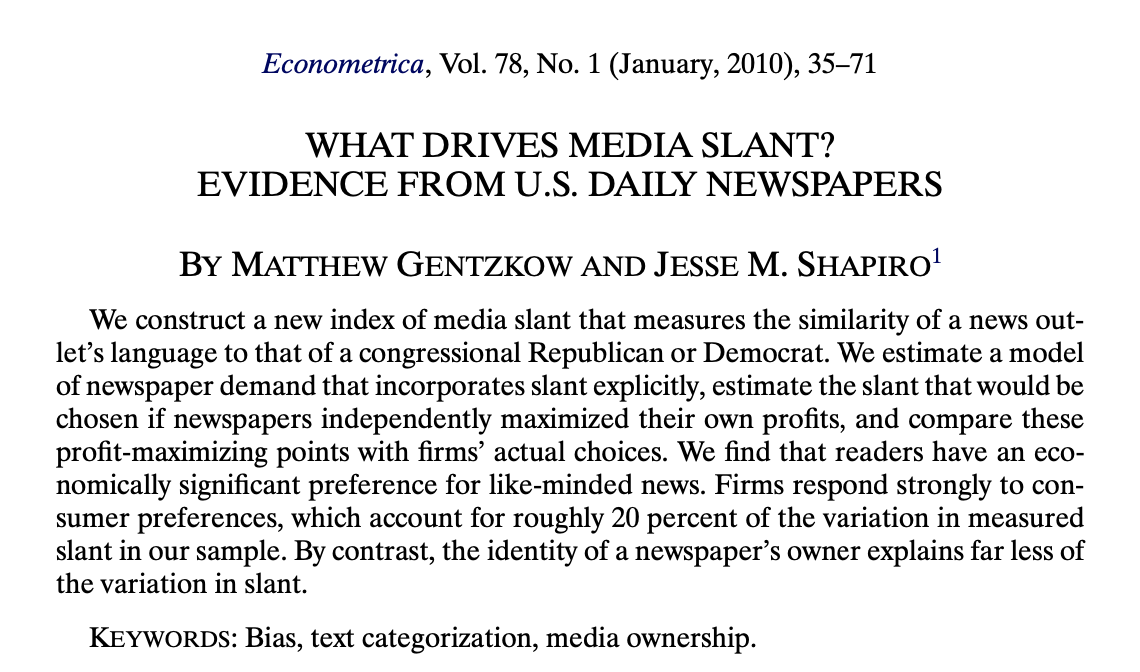
\includegraphics[scale=0.6]{figures/gentzgow_shapiro}
              
 \end{figure}

\end{frame}
%----------------------------------------------------------------------%
\begin{frame}[fragile]
\frametitle{Text as Data: Motivation}
\framesubtitle{Gentzkow and Shapiro: What drives media slant?  Evidence from
U.S. daily newspapers ({\it Econometrica}, 2010)}

\begin{itemize}
\item Build an economic model for newspaper demand that incorporates political partisanship (\rd Republican \bk vs \bl Democrat\bk)


 
\begin{itemize}
\item What would be independent profit-maximizing ``slant''?
\item Compare this to slant estimated from newspaper text.
\end{itemize}


\item use data from Congress to isolate the phrases
\item Compare phrase frequencies in the newspaper with phrase frequencies in the 2005 Congressional Record to identify whether the newspaper’s language is more similar to that of a congressional Republican or a congressional Democrat

\end{itemize}
\begin{table}[H]
\begin{tabular}{cc}
{\rd Republican}       & {\bl Democratic}      \\
\hline \\
death tax        & estate tax      \\
tax relief       & tax break       \\
personal account & private account \\
war on terror    & war in Iraq    
\end{tabular}
\end{table}
\end{frame}

%----------------------------------------------------------------------%

\begin{frame}[fragile]
\frametitle{Text as Data: Motivation}


  \begin{figure}[H] \centering
            \captionsetup{justification=centering}
              
\includegraphics[scale=0.5]{figures/Tetlock.png}
              
 \end{figure}

\end{frame}


%----------------------------------------------------------------------%
\subsection{Tokenization}
%----------------------------------------------------------------------%
\begin{frame}[fragile]
\frametitle{Information Retrieval and Tokenization}

\begin{itemize}


\item A passage in `{\it As You Like It}' from Shakepeare:

\medskip

~~~ {\sg All the world's a stage,\\
~~~ and all the men and women merely players:\\
~~~ they have their exits and their entrances;\\
~~~ and one man in his time plays many parts...}


\medskip
\item What the econometrian sees:

\medskip
\vspace{-.4cm}{\sg
\begin{verbatim}
   world stage men women play exit entrance time 
       1     1   2     1    2    1        1    1 
\end{verbatim}}

\medskip
\item This is the {\nv Bag-of-Words} representation of text.
\end{itemize}
\end{frame}


%----------------------------------------------------------------------%
\begin{frame}[fragile]
\frametitle{Possible tokenization steps} 

\begin{itemize}


\item Remove words that are super rare {\gr (in say $<\frac{1}{2}$\%, or $<15\%$ of docs; this is application specific)}.
 For example, if {\nv Argentine} occurs only once, it's useless for comparing documents.


\item Stemming:  `{\nv tax}' $\leftarrow$   taxing,  taxes, taxation, taxable, ... 

{\gr A stemmer cuts words to their root with a mix of rules and estimation.`Porter' is standard for English. }



\item  Remove a list of {\nv stop words} containing  irrelevant tokens.

{\gr ~~~~~If, and, but, who, what, the, they, their, a, or, ...}

{\nv Be careful: one person's stopword is another's key term.}


\item Convert to lowercase, drop numbers, punctuation, etc ...\\
{\gr Always application specific: e.g., don't drop {\tt :-)} from tweets.}
\end{itemize}


\end{frame}


%----------------------------------------------------------------------%
\begin{frame}[fragile]
\frametitle{The $n$-gram language model}

\begin{itemize}



\item An $n$-gram language model is one that describes a dialect through transition probabilities on $n$ consecutive words.

\medskip

\item An {\theme $n$-gram tokenization} counts length-$n$ sequences of words.\\
{\sg A unigram is a word, bigrams are transitions between words.}\\
{\gr e.g., {\tt world.stage}, {\tt stage.men}, {\tt men.women}, {\tt women.play}, ...}

\medskip

\item This can give you rich language data, but be careful: $n$-gram token vocabularies are very high dimensional ($p^n$)
\medskip
\item  More generally, you may have domain specific `clauses' that you wish to tokenize.
\medskip
\item  There is always a trade-off between complexity and generality. 
\medskip
\item {\theme Often best to just count words.}

\end{itemize}

\end{frame}
%----------------------------------------------------------------------%
\subsection{Tokenization Demo}
%----------------------------------------------------------------------%
\begin{frame}[fragile]
\frametitle{Tokenization Demo}

\begin{scriptsize}


\begin{Shaded}
\begin{Highlighting}[]
\CommentTok{\#\# the tm library (and related plugins) is R\textquotesingle{}s ecosystem for text mining.}
\CommentTok{\#\# for an intro see http://cran.r{-}project.org/web/packages/tm/vignettes/tm.pdf}
\KeywordTok{library}\NormalTok{(tm) }
\NormalTok{notes\textless{}{-}}\KeywordTok{readPDF}\NormalTok{(}\DataTypeTok{control =} \KeywordTok{list}\NormalTok{(}\DataTypeTok{text =} \StringTok{"{-}layout {-}enc UTF{-}8"}
  \NormalTok{))(}\DataTypeTok{elem=}\KeywordTok{list}\NormalTok{(}\DataTypeTok{uri=}\StringTok{"\textasciitilde{}/Papers/Beauty\_Hamermesh.pdf"}\NormalTok{), }\DataTypeTok{id=}\NormalTok{fname, }
  \DataTypeTok{language=}\StringTok{\textquotesingle{}en\textquotesingle{}}\NormalTok{)}
writeLines(content(notes)[1]) 
\end{Highlighting}
\end{Shaded}
\end{scriptsize}
\begin{tiny}



\begin{verbatim}
     ARTICLE IN PRESS
                                  Economics of Education Review 24 (2005) 369–376
                                                                                               www.elsevier.com/locate/econedurev
Beauty in the classroom: instructors’ pulchritude and putative
                                         pedagogical productivity
                                     Daniel S. Hamermesh, Amy Parker
                              Department of Economics, University of Texas, Austin, TX 78712-1173, USA
                                            Received 14 June 2004; accepted 21 July 2004
Abstract
   Adjusted for many other determinants, beauty affects earnings; but does it lead directly to the differences in
productivity that we believe generate earnings differences? We take a large sample of student instructional ratings for a
group of university teachers and acquire six independent measures of their beauty, and a number of other descriptors of
them and their classes. Instructors who are viewed as better looking receive higher instructional ratings, with the impact
of a move from the 10th to the 90th percentile of beauty being substantial. This impact exists within university
departments and even within particular courses, and is larger for male than for female instructors. Disentangling
whether this outcome represents productivity or discrimination is, as with the issue generally, probably impossible.
\end{verbatim}
\end{tiny}
\end{frame}
%----------------------------------------------------------------------%
\begin{frame}[fragile]
\frametitle{Tokenization Demo}

\begin{scriptsize}
\begin{Shaded}
\begin{Highlighting}[]
\KeywordTok{content}\NormalTok{(notes) \textless{}{-}}\KeywordTok{iconv}\NormalTok{(}\KeywordTok{content}\NormalTok{(notes), }\DataTypeTok{from=}\StringTok{"UTF{-}8"}\NormalTok{, }\DataTypeTok{to=}\StringTok{"ASCII"}\NormalTok{, }\DataTypeTok{sub=}\StringTok{""}\NormalTok{)}

\NormalTok{docs \textless{}{-}}\StringTok{ }\KeywordTok{Corpus}\NormalTok{(}\KeywordTok{VectorSource}\NormalTok{(notes))}

\KeywordTok{names}\NormalTok{(docs) \textless{}{-}}\StringTok{ }\KeywordTok{names}\NormalTok{(notes) }

\CommentTok{\#\# you can then do some cleaning here}
\CommentTok{\#\# tm\_map just maps some function to every document in the corpus}
\NormalTok{docs \textless{}{-}}\StringTok{ }\KeywordTok{tm\_map}\NormalTok{(docs, }\KeywordTok{content\_transformer}\NormalTok{(tolower)) }\CommentTok{\#\# make everything lowercase}
\NormalTok{docs \textless{}{-}}\StringTok{ }\KeywordTok{tm\_map}\NormalTok{(docs, }\KeywordTok{content\_transformer}\NormalTok{(removeNumbers)) }\CommentTok{\#\# remove numbers}
\NormalTok{docs \textless{}{-}}\StringTok{ }\KeywordTok{tm\_map}\NormalTok{(docs, }\KeywordTok{content\_transformer}\NormalTok{(removePunctuation)) }\CommentTok{\#\# remove punctuation}
\CommentTok{\#\# remove stopword. } 
\CommentTok{\#\#be careful with this: one\textquotesingle{}s stopwords are anothers keywords.}
\CommentTok{\# you could also do stemming; I don\textquotesingle{}t bother here.}
\NormalTok{docs \textless{}{-}}\StringTok{ }\KeywordTok{tm\_map}\NormalTok{(docs, }\KeywordTok{content\_transformer}\NormalTok{(removeWords), }\KeywordTok{stopwords}\NormalTok{(}\StringTok{"SMART"}\NormalTok{))}

\NormalTok{docs \textless{}{-}}\StringTok{ }\KeywordTok{tm\_map}\NormalTok{(docs, }\KeywordTok{content\_transformer}\NormalTok{(stripWhitespace)) }\CommentTok{\#\# remove excess white{-}space}
\end{Highlighting}
\end{Shaded}


\end{scriptsize}

\end{frame}
%----------------------------------------------------------------------%
\begin{frame}[fragile]
\frametitle{Tokenization Demo}


\begin{scriptsize}

\begin{Shaded}
\begin{Highlighting}[]
\CommentTok{\#\# create a doc{-}term{-}matrix}
\NormalTok{dtm \textless{}{-}}\StringTok{ }\KeywordTok{DocumentTermMatrix}\NormalTok{(docs)}
\NormalTok{dtm }
\end{Highlighting}
\end{Shaded}


\end{scriptsize}
\begin{tiny}



\begin{verbatim}
## <<DocumentTermMatrix (documents: 8, terms: 913)>>
## Non-/sparse entries: 1555/5749
## Sparsity           : 79%
## Maximal term length: 30
## Weighting          : term frequency (tf)
\end{verbatim}

\end{tiny}
\begin{scriptsize}

\begin{Shaded}
\begin{Highlighting}[]
\NormalTok{dtm \textless{}{-}}\StringTok{ }\KeywordTok{removeSparseTerms}\NormalTok{(dtm, }\FloatTok{0.75}\NormalTok{)}
\NormalTok{dtm }
\end{Highlighting}
\end{Shaded}

\end{scriptsize}
\begin{tiny}
\begin{verbatim}
## <<DocumentTermMatrix (documents: 8, terms: 156)>>
## Non-/sparse entries: 650/598
## Sparsity           : 48%
## Maximal term length: 15
## Weighting          : term frequency (tf)
\end{verbatim}
\end{tiny}
\end{frame}
%----------------------------------------------------------------------%
\begin{frame}[fragile]
\frametitle{Tokenization Demo}

\begin{scriptsize}


\begin{Shaded}
\begin{Highlighting}[]
\CommentTok{\#\# You can inspect them:}
\KeywordTok{inspect}\NormalTok{(dtm[}\DecValTok{1}\OperatorTok{:}\DecValTok{5}\NormalTok{,}\DecValTok{1}\OperatorTok{:}\DecValTok{8}\NormalTok{])}
\end{Highlighting}
\end{Shaded}
\end{scriptsize}
\begin{tiny}

\begin{verbatim}
## <<DocumentTermMatrix (documents: 5, terms: 8)>>
## Non-/sparse entries: 26/14
## Sparsity           : 35%
## ...
## Docs academic article beauty becker behavior biddle class classes
##    1        1       1      9      1        1      2     1       1
##    2        2       1      7      0        1      0     5       5
##    3        0       1      6      0        0      0     0       1
\end{verbatim}

\end{tiny}

\begin{scriptsize}
\begin{Shaded}
\begin{Highlighting}[]
\CommentTok{\#\# find words with greater than a min count}
\KeywordTok{findFreqTerms}\NormalTok{(dtm,}\DecValTok{50}\NormalTok{)}
\end{Highlighting}
\end{Shaded}

\end{scriptsize}
\begin{tiny}

\begin{verbatim}
## [1] "beauty"  "ratings"
\end{verbatim}

\end{tiny}
\begin{scriptsize}


\begin{Shaded}
\begin{Highlighting}[]
\CommentTok{\#\# or grab words whose count correlates with given words}
\KeywordTok{findAssocs}\NormalTok{(dtm, }\StringTok{"beauty"}\NormalTok{, }\FloatTok{.7}\NormalTok{) }
\end{Highlighting}
\end{Shaded}
\end{scriptsize}
\begin{tiny}


\begin{verbatim}
## $beauty
##  equation    effect     basic  positive     table perceived   results potential 
##      0.86      0.83      0.79      0.77      0.77      0.77      0.73      0.72 
##   problem   effects   instruc 
##      0.72      0.71      0.70
\end{verbatim}
\end{tiny}

\end{frame}
%----------------------------------------------------------------------%
\section{Text Regression}
%----------------------------------------------------------------------%
\begin{frame}
\frametitle{Text Regression}

\begin{itemize}
\item Once you have text in a numeric format, we can use all the tools we learned so far

\medskip

\item For example: Classify emails into spam

\begin{align}
\mr{logit}\left[{\tt spam} \right] = \alpha + f \beta
\end{align}
\item where $f_i=\frac{x_i}{\sum_j x_{ij}}$ are the normalized text counts

\end{itemize}

\end{frame}

%----------------------------------------------------------------------%
\subsection{Text Regression: Example}
%----------------------------------------------------------------------%
\begin{frame}[fragile]
\frametitle{Text Regression: Example (Gentzkow and Shapiro)}
\begin{scriptsize}



\begin{Shaded}
\begin{Highlighting}[]
\CommentTok{\#load packages}
\KeywordTok{library}\NormalTok{(textir) }
\CommentTok{\#load data}
\KeywordTok{data}\NormalTok{(congress109)}
\NormalTok{congress109Counts[}\KeywordTok{c}\NormalTok{(}\StringTok{"Barack Obama"}\NormalTok{,}\StringTok{"John Boehner"}\NormalTok{),}\DecValTok{995}\OperatorTok{:}\DecValTok{998}\NormalTok{]}
\end{Highlighting}
\end{Shaded}

\end{scriptsize}
\begin{tiny}


\begin{verbatim}
## 2 x 4 sparse Matrix of class "dgCMatrix"
##              stem.cel natural.ga hurricane.katrina trade.agreement
## Barack Obama        .          1                20               7
## John Boehner        .          .                14               .
\end{verbatim}

\end{tiny}
\begin{scriptsize}


\begin{Shaded}
\begin{Highlighting}[]
\NormalTok{congress109Ideology[}\DecValTok{1}\OperatorTok{:}\DecValTok{4}\NormalTok{,}\DecValTok{1}\OperatorTok{:}\DecValTok{5}\NormalTok{]}
\end{Highlighting}
\end{Shaded}
\end{scriptsize}
\begin{tiny}


\begin{verbatim}
##                            name party state chamber  repshare
## Chris Cannon       Chris Cannon     R    UT       H 0.7900621
## Michael Conaway Michael Conaway     R    TX       H 0.7836028
## Spencer Bachus   Spencer Bachus     R    AL       H 0.7812933
## Mac Thornberry   Mac Thornberry     R    TX       H 0.7776520
\end{verbatim}
\end{tiny}
\end{frame}
%----------------------------------------------------------------------%
\begin{frame}[fragile]
\frametitle{Text Regression: Example (Gentzkow and Shapiro)}

\begin{scriptsize}


\begin{Shaded}
\begin{Highlighting}[]
\KeywordTok{require}\NormalTok{(}\StringTok{"wordcloud"}\NormalTok{)}
\KeywordTok{wordcloud}\NormalTok{(}\DataTypeTok{words =} \KeywordTok{colnames}\NormalTok{(congress109Counts), }
          \DataTypeTok{freq =} \KeywordTok{colSums}\NormalTok{(congress109Counts),}
          \DataTypeTok{min.freq =} \DecValTok{100}\NormalTok{,}
          \DataTypeTok{scale =} \KeywordTok{c}\NormalTok{(}\DecValTok{3}\NormalTok{, }\FloatTok{0.1}\NormalTok{), }\DataTypeTok{max.words=}\DecValTok{200}\NormalTok{, }
          \DataTypeTok{random.order=}\OtherTok{FALSE}\NormalTok{, }\DataTypeTok{rot.per=}\FloatTok{0.35}\NormalTok{, }
          \DataTypeTok{colors=}\KeywordTok{brewer.pal}\NormalTok{(}\DecValTok{8}\NormalTok{, }\StringTok{"Set1"}\NormalTok{))}
\end{Highlighting}
\end{Shaded}
\end{scriptsize}

  \begin{figure}[H] \centering
            \captionsetup{justification=centering}
              
\includegraphics[scale=0.5]{figures/unnamed-chunk-3-1.pdf}
              
 \end{figure}


\end{frame}
%----------------------------------------------------------------------%
\begin{frame}[fragile]
\frametitle{Text Regression: Wordle (Wordclouds)}


\begin{scriptsize}


\begin{Shaded}
\begin{Highlighting}[]
\KeywordTok{tail}\NormalTok{(}\KeywordTok{colSums}\NormalTok{(congress109Counts))}
\end{Highlighting}
\end{Shaded}
\end{scriptsize}
\begin{tiny}



\begin{verbatim}
##          stem.cel        natural.ga hurricane.katrina   trade.agreement 
##              1699              1792              2020              2329 
## appropriation.bil   american.people 
##              2357              6256
\end{verbatim}
\end{tiny}

\begin{scriptsize}



\begin{Shaded}
\begin{Highlighting}[]
\KeywordTok{wordcloud}\NormalTok{(}\DataTypeTok{words =} \KeywordTok{colnames}\NormalTok{(congress109Counts), }
          \DataTypeTok{freq =} \KeywordTok{colSums}\NormalTok{(congress109Counts),}
          \DataTypeTok{min.freq =} \DecValTok{1000}\NormalTok{, }
          \DataTypeTok{scale =} \KeywordTok{c}\NormalTok{(}\DecValTok{3}\NormalTok{, }\FloatTok{0.1}\NormalTok{), }\DataTypeTok{max.words=}\DecValTok{30}\NormalTok{, }
          \DataTypeTok{random.order=}\OtherTok{FALSE}\NormalTok{, }\DataTypeTok{rot.per=}\FloatTok{0.35}\NormalTok{, }
          \DataTypeTok{colors=}\KeywordTok{brewer.pal}\NormalTok{(}\DecValTok{8}\NormalTok{, }\StringTok{"Set1"}\NormalTok{))}
\end{Highlighting}
\end{Shaded}

\end{scriptsize}


  \begin{figure}[H] \centering
            \captionsetup{justification=centering}
              
\includegraphics[scale=0.5]{figures/unnamed-chunk-5-1.pdf}
              
 \end{figure}



\end{frame}
%----------------------------------------------------------------------%
\begin{frame}[fragile]
\frametitle{Text Regression}

\begin{itemize}
  \item We can use {\tt LASSO}
\end{itemize}
\begin{scriptsize}

\begin{Shaded}
\begin{Highlighting}[]
\NormalTok{f \textless{}{-}}\StringTok{ }\NormalTok{congress109Counts}
\NormalTok{y \textless{}{-}}\StringTok{ }\NormalTok{congress109Ideology}\OperatorTok{$}\NormalTok{repshare}
\CommentTok{\# lasso }
\NormalTok{lassoslant \textless{}{-}}\StringTok{ }\KeywordTok{cv.gamlr}\NormalTok{(congress109Counts}\OperatorTok{\textgreater{}}\DecValTok{0}\NormalTok{, y)}
\NormalTok{B \textless{}{-}}\StringTok{ }\KeywordTok{coef}\NormalTok{(lassoslant}\OperatorTok{$}\NormalTok{gamlr)[}\OperatorTok{{-}}\DecValTok{1}\NormalTok{,]}
\KeywordTok{head}\NormalTok{(}\KeywordTok{sort}\NormalTok{(}\KeywordTok{round}\NormalTok{(B[B}\OperatorTok{!=}\DecValTok{0}\NormalTok{],}\DecValTok{4}\NormalTok{)),}\DecValTok{10}\NormalTok{)}
\end{Highlighting}
\end{Shaded}

\end{scriptsize}
\begin{tiny}


\begin{verbatim}
##    congressional.black.caucu                 family.value 
##                      -0.0839                      -0.0443 
##        issue.facing.american           voter.registration 
##                      -0.0324                      -0.0298 
##      minority.owned.business            strong.opposition 
##                      -0.0284                      -0.0264 
##                  civil.right        universal.health.care 
##                      -0.0259                      -0.0254 
## congressional.hispanic.caucu          ohio.electoral.vote 
##                      -0.0187                      -0.0183
\end{verbatim}
\end{tiny}

\end{frame}
%----------------------------------------------------------------------%
\begin{frame}[fragile]
\frametitle{Text Regression}

\begin{scriptsize}

\begin{Shaded}
\begin{Highlighting}[]
\KeywordTok{tail}\NormalTok{(}\KeywordTok{sort}\NormalTok{(}\KeywordTok{round}\NormalTok{(B[B}\OperatorTok{!=}\DecValTok{0}\NormalTok{],}\DecValTok{4}\NormalTok{)),}\DecValTok{10}\NormalTok{)}
\end{Highlighting}
\end{Shaded}

\end{scriptsize}
\begin{tiny}

\begin{verbatim}
##         illegal.alien        percent.growth   illegal.immigration 
##                0.0079                0.0083                0.0087 
##            global.war          look.forward            war.terror 
##                0.0098                0.0099                0.0114 
##      private.property        action.lawsuit          human.embryo 
##                0.0133                0.0142                0.0226 
## million.illegal.alien 
##                0.0328
\end{verbatim}


\end{tiny}

\end{frame}
%----------------------------------------------------------------------%
\section{Topic Models}
%----------------------------------------------------------------------%
\begin{frame}
\frametitle{Topic Models}

\begin{itemize}
\item Text is super high dimensional
\medskip
\item there is often abundant {\it unlabeled} text
\medskip
\item Some times unsupervized factor model is a popular and useful strategy with text data
\medskip
\item You can first fit a factor model to a giant corpus and use these factors for supervised learning on a subset of labeled documents.
\medskip
\item The unsupervised dimension reduction facilitates the supervised learning
\end{itemize}
\end{frame}
%----------------------------------------------------------------------%
\begin{frame}
\frametitle{Topic Models: Example}

\begin{itemize}


\item We have 6166 reviews, with an average length of 90 words per review, \url{we8there.com}. 
\medskip
\item A useful feature of these reviews is that they contain both text and a multidimensional rating on overall experience, atmosphere, food, service, and value. 
\medskip
\item For example, one user submitted a glowing review for Waffle House \#1258 in Bossier City, Louisiana: 
\medskip
{\tt \it 
I normally would not revue a Waffle House but this one deserves it. The workers, Amanda, Amy, Cherry, James and J.D. were the most pleasant crew I have seen. While it was only lunch, B.L.T. and chili, it was great. The best thing was the 50’ s rock and roll music, not to loud not to soft. This is a rare exception to what you all think a Waffle House is. Keep up the good work. \\
Overall: 5, Atmosphere: 5, Food: 5, Service: 5, Value: 5. 
}
\end{itemize}
\end{frame}
%----------------------------------------------------------------------%
\begin{frame}[fragile]
\frametitle{Topic Models: Example}
\begin{itemize}


\item After cleaning and Porter stemming, we are left with a vocabulary of 2640 bigrams. 
\item For example, the first review in the document-term matrix has nonzero counts on bigrams indicating a pleasant meal at a rib joint: 
\end{itemize}

\begin{scriptsize}

\begin{Shaded}
\begin{Highlighting}[]
\CommentTok{\#load packages}
\KeywordTok{library}\NormalTok{(textir) }
\CommentTok{\#load data}
\KeywordTok{data}\NormalTok{(we8there)}
\NormalTok{x \textless{}{-}}\StringTok{ }\NormalTok{we8thereCounts}
\NormalTok{x[}\DecValTok{1}\NormalTok{,x[}\DecValTok{1}\NormalTok{,]}\OperatorTok{!=}\DecValTok{0}\NormalTok{]}
\end{Highlighting}
\end{Shaded}

\end{scriptsize}
\begin{tiny}



\begin{verbatim}
## even though larg portion  mouth water     red sauc    babi back     back rib chocol mouss 
##           1            1            1            1            1            1            1 
## veri satisfi 
##            1 
\end{verbatim}
\end{tiny}
\end{frame}
%----------------------------------------------------------------------%
\begin{frame}[fragile]
\frametitle{Topic Models: Example}

\begin{itemize}


\item We can apply PCA to get a factor representation of the review text. 
\item  PC1 looks like it will be big and positive for positive reviews, 

\begin{scriptsize}

\begin{Shaded}
\begin{Highlighting}[]
\NormalTok{pca \textless{}{-}}\StringTok{ }\KeywordTok{prcomp}\NormalTok{(x, }\DataTypeTok{scale=}\OtherTok{TRUE}\NormalTok{) }\CommentTok{\# can take a long time}

\KeywordTok{tail}\NormalTok{(}\KeywordTok{sort}\NormalTok{(pca}\OperatorTok{$}\NormalTok{rotation[,}\DecValTok{1}\NormalTok{]))}
\end{Highlighting}
\end{Shaded}

\end{scriptsize}
\begin{tiny}

\begin{verbatim}
##     food great     staff veri     excel food high recommend     great food 
##    0.007386860    0.007593374    0.007629771    0.007821171    0.008503594 
##     food excel 
##    0.008736181
\end{verbatim}

\end{tiny}


\begin{scriptsize}

\item while PC4 will be big and negative 
\begin{Shaded}
\begin{Highlighting}[]
\KeywordTok{tail}\NormalTok{(}\KeywordTok{sort}\NormalTok{(pca}\OperatorTok{$}\NormalTok{rotation[,}\DecValTok{4}\NormalTok{]))}
\end{Highlighting}
\end{Shaded}
\end{scriptsize}
\begin{tiny}

\begin{verbatim}
##   order got after minut  never came   ask check readi order drink order 
##  0.05918712  0.05958572  0.06099509  0.06184512  0.06776281  0.07980788
\end{verbatim}
\end{tiny}




\end{itemize}
\end{frame}

%----------------------------------------------------------------------%
\subsection{PCA}
%----------------------------------------------------------------------%
\begin{frame}
\frametitle{Principal Component Analysis}

\begin{itemize}

  \item Dimensionality via main components

  \begin{align}
  X = (x_1 , x_2 , \dots , x_n )_{N \times K}
  \end{align}

  \item Factor: 

  \begin{align}
  F = X\delta \,\,\,\delta \in K
  \end{align}


  \item Idea: summarize the K variables in a single (F).
  \item Vocab: the coefficients of $\delta$ are the loadings: how much 'matters' each x s in the factor.
  \item Dimensionality: summarize the original K variables in a few $q <K$ factors.
  \end{itemize}

\end{frame}



%----------------------------------------------------------------------%
\begin{frame}
\frametitle{Algebra Review}

\begin{itemize}

\item Let $A_{m\times m}$. It exists 
\begin{itemize}
  \item a scalar $\lambda$ such that $Ax = \lambda x$ for a vector $m\times 1$, $x \neq 0$ is an eigenvalue of A. 
  \item and a vector $x$ is an eigenvector of A corresponding to the eigenvalue $\lambda$.
\end{itemize}

\item $A_{m\times m}$ with eigenvalues $\lambda_1, \lambda_2,\dots,\lambda_m$, then:

\begin{align}
tr(A) &= \sum_{i=1}^m \lambda_i \\
det(A) &= \Pi_{i=1}^m \lambda_i
\end{align}

\item If $A_{m\times m}$ has $m$ different eigenvalues, then the associated eigenvectors are all linearly independent.
\item Spectral decomposition: $A = P\Lambda P$, where $\Lambda = diag(\lambda_1, \dots \lambda_n )$ and $P$ is the matrix whose columns are the corresponding eigenvectors.
\end{itemize}

\end{frame}


%----------------------------------------------------------------------%
\begin{frame}
\frametitle{Factors via main components}

\begin{itemize}


\item $x_1, x_2, \dots, x_K$ , K vectors of N observations each.
\medskip
\item Factor: $F = X\delta$
\medskip
\item What is the 'best' linear combination of $x_1, x_2, \dots, x_K$ ?
\medskip
\item Best? Maximum variance. Why? The one that best reproduces variability original of all xs

\end{itemize}
\end{frame}
%----------------------------------------------------------------------%
\begin{frame}
\frametitle{Factors via main components}

\begin{itemize}
  \item Let
  \begin{itemize}
    \item $X = (x_1 , \dots , x_K)_{N \times K}$  , 
    \item $\Sigma V(X)$ 
    \item $\delta \in K$
 \end{itemize}
  \medskip
  \item $F = X\delta$ is a linear combination of $X$, with $V (X\delta) = \delta' \Sigma \delta$.
  \medskip
  \item Let's set up the problem as 
  \begin{align}
  \underset{\delta}{max}\,\,\, \delta' \Sigma \delta
  \end{align}
 \begin{itemize}
  \item It is obvious that the solution is to bring $\delta$ to infinity. 
 \end{itemize}
\end{itemize}
 \end{frame}
%----------------------------------------------------------------------%
\begin{frame}
\frametitle{Factors via main components}

\begin{itemize}
\item Let's "fix" the problem by normalizing $\delta$

\begin{align}
\underset{\delta}{max} \delta' \Sigma \delta \\ \nonumber
\text{subject to}  \\ \nonumber
\delta' \delta = 1 \nonumber
\end{align}
\item Let us call the solution to this problem $\delta^*$. 
\medskip
\item $F^* = X\delta^*$ is the 'best' linear combination of X. 

\end{itemize}
\end{frame}


%----------------------------------------------------------------------%
\begin{frame}
\frametitle{Factors via main components}

\begin{itemize}
\item Result: $\delta^*$ is the eigenvector corresponding to the largest eigenvalue of $\Sigma = V (X)$.
\medskip
\item $F^* = X\delta^*$ is the first principal component of $X$.
\medskip
\item Intuition: $X$ has $K$ columns and $Y = X\delta$ has only one. The factor built with the first principal component is the best way to represent the K variables of X using a single single variable.
\end{itemize}

\end{frame}

\begin{comment}
%----------------------------------------------------------------------%
\begin{frame}
\frametitle{Factors via main components}
Solution to the problem of the first principal component
Problem: max δ δ Σδ,
subject to δ δ = 1
Lagrange: L (δ, λ) = δ Σδ + λ (1 - δ δ). CPO:
Σ δ = λ δ
At the optimum, δ is the eigenvector corresponding to the eigenvalue λ of Σ. Premultiplying by δ and
remembering that δ δ = 1:
δ Σδ = λ
In order to maximize δ Σδ we must choose λ equal to the maximum eigenvalue of Σ and δ equal to
corresponding eigenvalue.
\end{frame}
%----------------------------------------------------------------------%
\begin{frame}
\frametitle{Factors via main components}
Factors such as unsupervised learning
Regression Y = Xβ + u. ˆY ≡ X
ˆ
β. Min ∑ (Y i - ˆY) 2
Learning is supervised: the discrepancy between Y and ˆY 'guides' learning.
The factor construction problem is unsupervised : we construct an index (the
factor) without ever seeing it.
We start with X N × K and end with F ∗
N × 1
= Xδ ∗
\end{frame}


\end{comment}
%----------------------------------------------------------------------%
\section{Review
 \& Next Steps}
%----------------------------------------------------------------------%
\begin{frame}
\frametitle{Review \& Next Steps}
  
\begin{itemize} 
   \item XGBOOST
   \bigskip
   \item XGBOOST demo
   \bigskip
  \item Text as data
    \bigskip  
  \item  Next class:  More on text as data


\bigskip  
\item Questions? Questions about software? 

\end{itemize}
\end{frame}

%----------------------------------------------------------------------%
\section{Further Readings}
%----------------------------------------------------------------------%
\begin{frame}
\frametitle{Further Readings}

\begin{itemize}

  \item Gentzkow, M., \& Shapiro, J. M. (2010). What drives media slant? Evidence from US daily newspapers. Econometrica, 78(1), 35-71.
  \medskip
  \item Friedman, J., Hastie, T., \& Tibshirani, R. (2001). The elements of statistical learning (Vol. 1, No. 10). New York: Springer series in statistics.
  \medskip
  \item James, G., Witten, D., Hastie, T., \& Tibshirani, R. (2013). An introduction to statistical learning (Vol. 112, p. 18). New York: springer.
  \medskip
  \item Taddy, M. (2019). Business data science: Combining machine learning and economics to optimize, automate, and accelerate business decisions. McGraw Hill Professional.

  
\end{itemize}

\end{frame}
%----------------------------------------------------------------------%
%----------------------------------------------------------------------%
\end{document}
%----------------------------------------------------------------------%
%----------------------------------------------------------------------%

